\documentclass[12pt,a4paper]{report}
% Packages for enhanced functionality
\usepackage[utf8]{inputenc}
\usepackage[T1]{fontenc}
\usepackage{graphicx} % For including images
\usepackage{geometry} % For page layout
\usepackage{hyperref} % For clickable links and references
\usepackage{fancyhdr} % For custom headers and footers
\usepackage{titlesec} % For section title formatting
\usepackage{float} \usepackage{circuitikz}
\usepackage{caption}
\usepackage{siunitx}
\usepackage{amsmath}
\usepackage{subcaption}
\usepackage{booktabs}
\newcommand{\vecb}[1]{\mathbf{#1}}
\newcommand{\brak}[1]{\ensuremath{\left(#1\right)}}
\newcommand{\cbrak}[1]{\ensuremath{\left\{#1\right\}}}
\newcommand{\abs}[1]{\left\vert#1\right\vert}
\newcommand{\norm}[1]{\left\lVert#1\right\rVert}
\providecommand{\sbrak}[1]{\ensuremath{{}\left[#1\right]}}
\providecommand{\lsbrak}[1]{\ensuremath{{}\left[#1\right.}}
\providecommand{\rsbrak}[1]{\ensuremath{{}\left.#1\right]}}
\providecommand{\brak}[1]{\ensuremath{\left(#1\right)}}
\providecommand{\lbrak}[1]{\ensuremath{\left(#1\right.}}
\providecommand{\rbrak}[1]{\ensuremath{\left.#1\right)}}
\providecommand{\cbrak}[1]{\ensuremath{\left\{#1\right\}}}
\providecommand{\lcbrak}[1]{\ensuremath{\left\{#1\right.}}
\providecommand{\rcbrak}[1]{\ensuremath{\left.#1\right\}}}
\hypersetup{
    colorlinks=true,  % Enable colored text links
    linkcolor=orange,    % Internal links (sections, table of contents, etc.)
    urlcolor=orange,     % External URLs
    citecolor=orange,    % Citations
    pdfborder={0 0 0} % Remove ugly default borders
}
\begin{document}
\title{\textbf{Experiment 1}\\
\LARGE{\textbf{ }}
\author{ Arjun Pavanje (EE24BTECH11005)}

\begin{center}
\end{center}
\vspace{30pt}
\begin{figure}[ht]
	\centering
	
\includegraphics[width = 100pt]{logo.png}\\
\end{figure}
\begin{center}
	Bachelor of Technology\\
	\vspace{10pt}
	Department of Electrical Engineering\\
\end{center}
}
\maketitle


Aim, Apparatus, theory, spicemodels, circuits, plots, conclusion
\section{Aim} To characterize the electrical behavior of diodes, BJTs, and MOSFETs by plotting their I-V characteristics through simulations (LTspice).
\section{Apparatus}
Laptop
\section{Theory}
\section{Procedure}
\subsection{Basic Procedure},
\begin{enumerate}
    \item Opening components menu,
    \begin{figure}[h!]
        \centering
        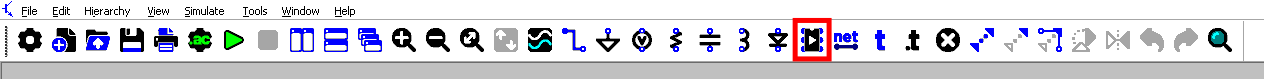
\includegraphics[width=0.7\linewidth]{figs/component-bar.png}
        \label{fig:placeholder}
    \end{figure}
    \item Modifying DC-Sweep settings,
    \begin{figure}[h!]
        \centering
        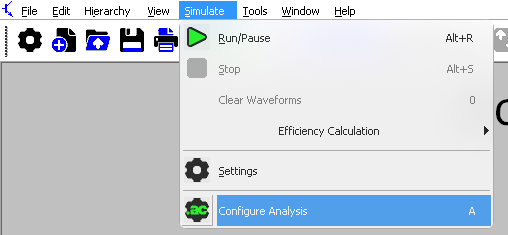
\includegraphics[width=0.5\linewidth]{figs/simulate.png}
        \label{fig:placeholder}
    \end{figure}
    \item Running simulation,
    \pagebreak
    \begin{figure}[h!]
        \centering
        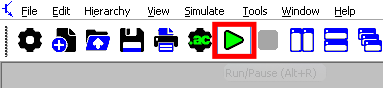
\includegraphics[width=0.5\linewidth]{figs/run.png}
        \label{fig:placeholder}
    \end{figure}
\end{enumerate}
\subsection{MOSFET}
\begin{enumerate}
    \item Select the MOSFET (shown in the figure) and 2 voltage sources.
    \begin{figure}[h!]
        \centering
        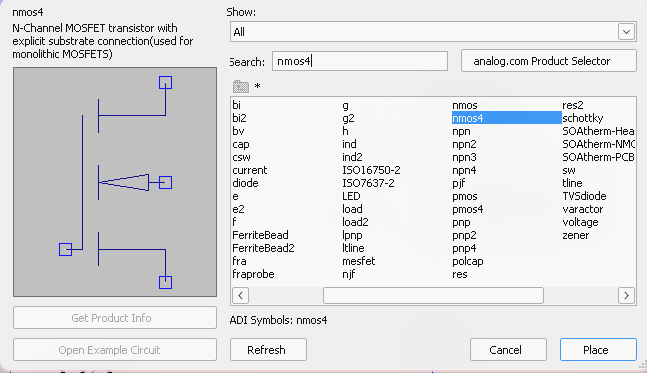
\includegraphics[width = 0.6\linewidth]{figs/component-nmos.png}
        \label{fig:placeholder}
    \end{figure}
    \item Select an appropriate commercially available model of the nmos,
    \begin{figure}[h!]
        \centering
        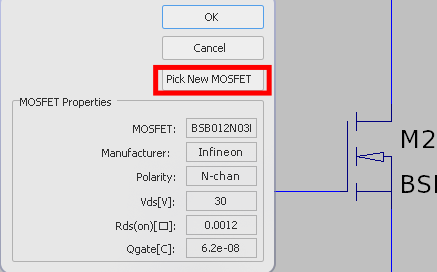
\includegraphics[width=0.5\linewidth]{figs/mosfet-model.png}
        \label{fig:placeholder}
    \end{figure}
    \item Connect the circuit as shown,
    \pagebreak
    \begin{figure}[h!]
        \centering
        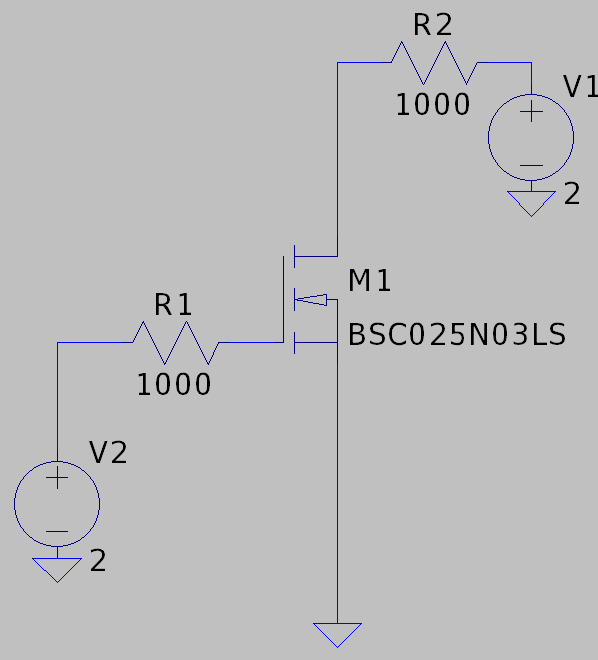
\includegraphics[width=0.5\linewidth]{figs/mosfet-circuit.png}
        \label{fig:placeholder}
    \end{figure}
    \item Configure DC sweep settings from the $Simulate$ bar. These were the settings used in this case,
  \begin{figure}[h!]
  \centering
  
  \begin{subfigure}[b]{0.45\textwidth}
    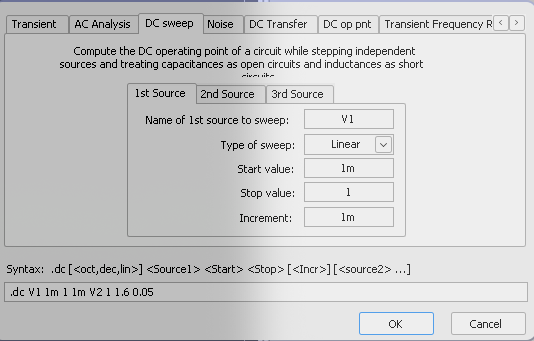
\includegraphics[width=\textwidth]{figs/mosfet-sweep-1.png}
  \end{subfigure}
  \begin{subfigure}[b]{0.45\textwidth}
    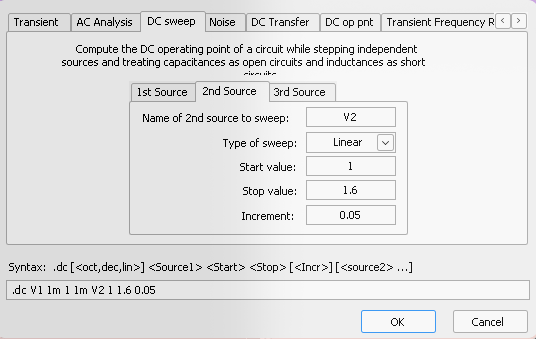
\includegraphics[width=\textwidth]{figs/mosfet-sweep-2.png}
  \end{subfigure}
  \label{fig:main}
\end{figure}
    
    \item Run the simulation
\end{enumerate}
\subsection{BJT}
\begin{enumerate}
    \item Select the BJT (shown in the figure), 2 resistors, 2 voltage sources.
    \pagebreak
    \begin{figure}[h!]
        \centering
        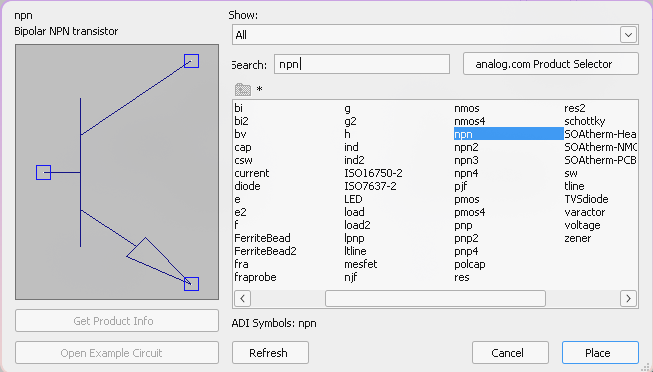
\includegraphics[width = 0.6\linewidth]{figs/component-bjt.png}
        \label{fig:placeholder}
    \end{figure}
    \item Select an appropriate commercially available model of the npn transistor,
    \begin{figure}[h!]
        \centering
        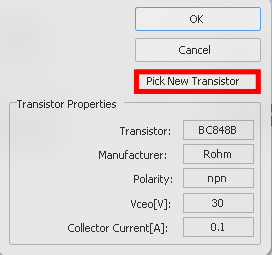
\includegraphics[width=0.5\linewidth]{figs/bjt-model.png}
        \label{fig:placeholder}
    \end{figure}
    \item Connect the circuit as shown,
    \begin{figure}[h!]
        \centering
        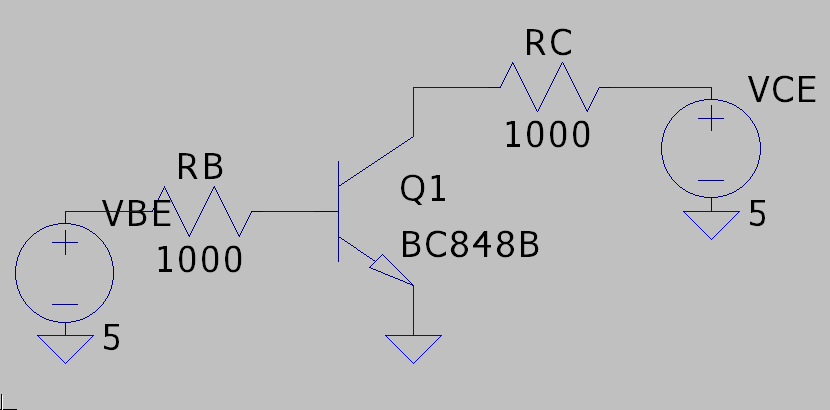
\includegraphics[width=0.5\linewidth]{figs/bjt-circuit.png}
        \label{fig:placeholder}
    \end{figure}
    \item Configure DC sweep settings from the $Simulate$ bar. These were the settings used in this case,
  \begin{figure}[h!]
  \centering
  
  \begin{subfigure}[b]{0.45\textwidth}
    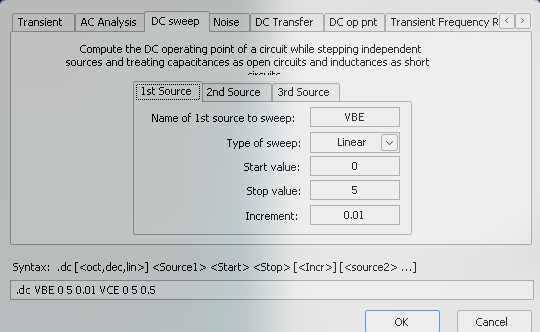
\includegraphics[width=\textwidth]{figs/bjt-sweep-1.png}
  \end{subfigure}
  \begin{subfigure}[b]{0.45\textwidth}
    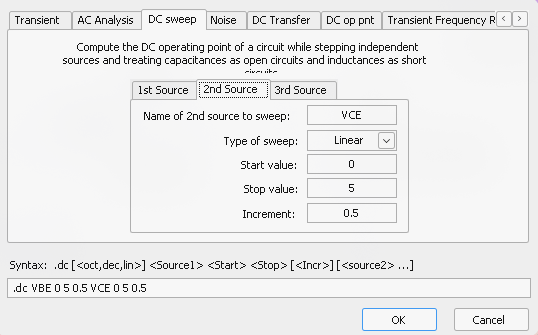
\includegraphics[width=\textwidth]{figs/bjt-sweep-2.png}
  \end{subfigure}
  \label{fig:main}
\end{figure}
    
    \item Run the simulationi
\end{enumerate}
\subsection{Diode}
\begin{enumerate}
    \item Select the diode (shown in the figure), a resistor, a voltage source.
    \begin{figure}[h!]
        \centering
        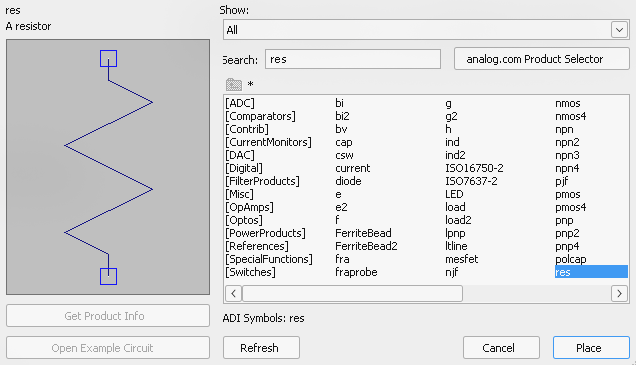
\includegraphics[width = 0.6\linewidth]{figs/component-diode.png}
        \label{fig:placeholder}
    \end{figure}
    \item Select an appropriate commercially available model of the npn transistor,
    \begin{figure}[h!]
        \centering
        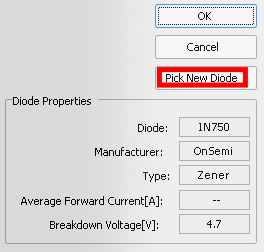
\includegraphics[width=0.3\linewidth]{figs/diode-model.png}
        \label{fig:placeholder}
    \end{figure}
    \item Connect the circuit as shown,
    \begin{figure}[h!]
        \centering
        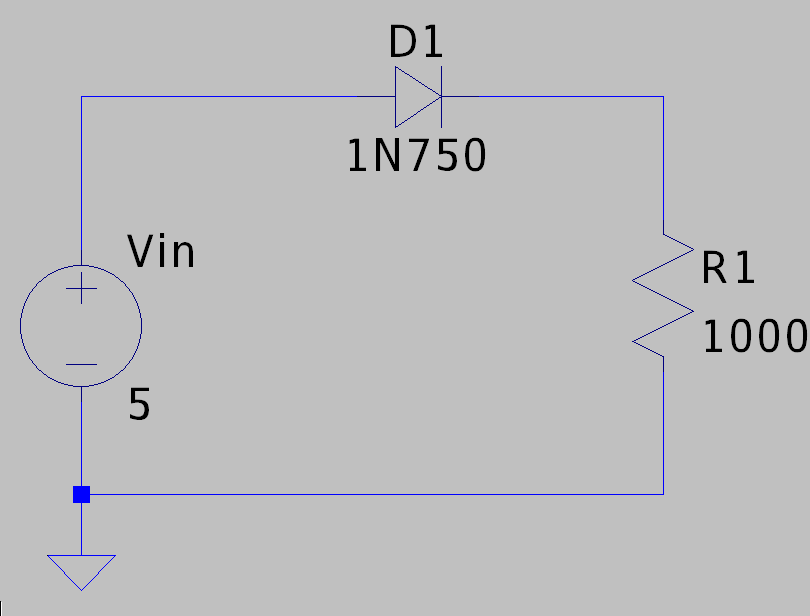
\includegraphics[width=0.5\linewidth]{figs/diode-circuit.png}
        \label{fig:placeholder}
    \end{figure}
    \item Configure DC sweep settings from the $Simulate$ bar. These were the settings used in this case,
    \begin{figure}[h!]
        \centering
        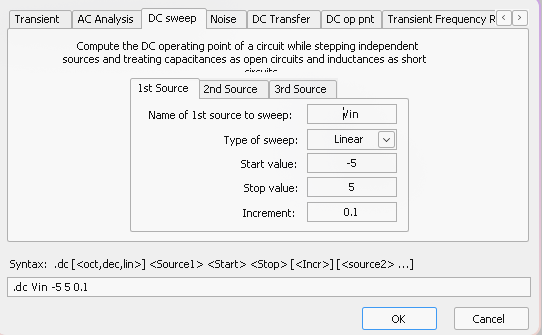
\includegraphics[width=0.5\linewidth]{figs/diode-sweep.png}
        \label{fig:placeholder}
    \end{figure}
    
    \item Run the simulation
\end{enumerate}
\section{Plots}
    \subsection{MOSFET}
    \begin{figure}[h!]
        \centering
        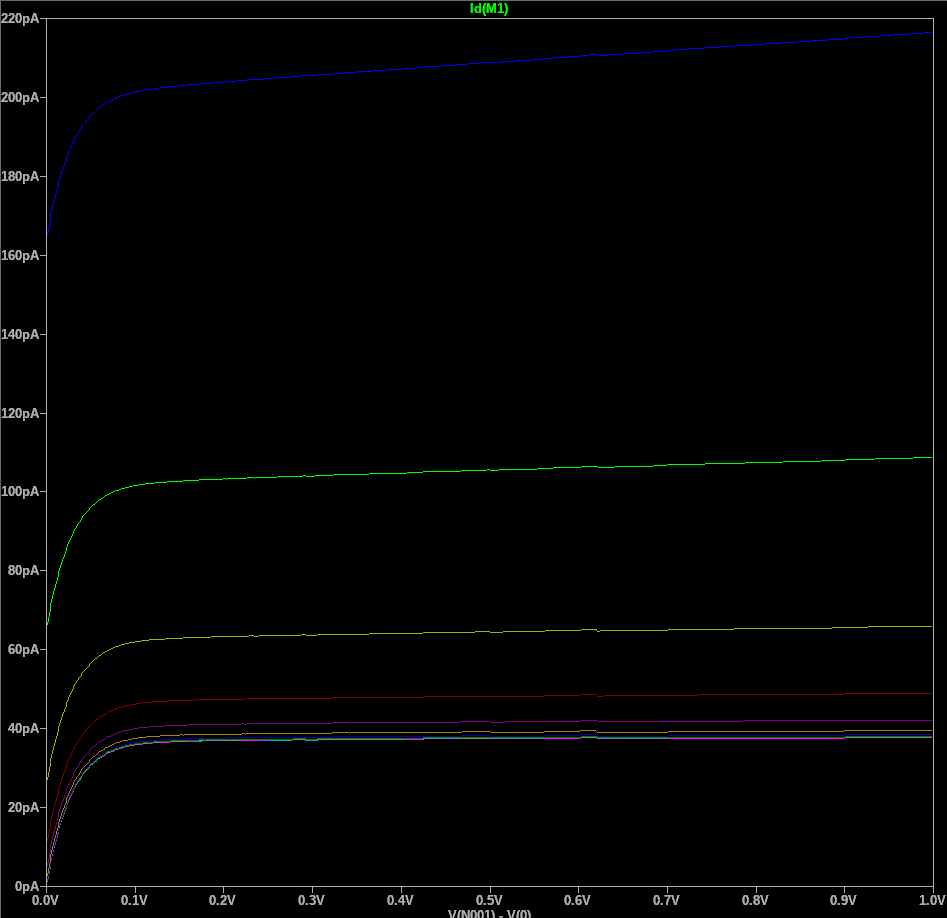
\includegraphics[width=1\linewidth]{figs/mosfet-plot.png}
    \end{figure}
    \subsection{BJT}
    \begin{figure}[h!]
        \centering
        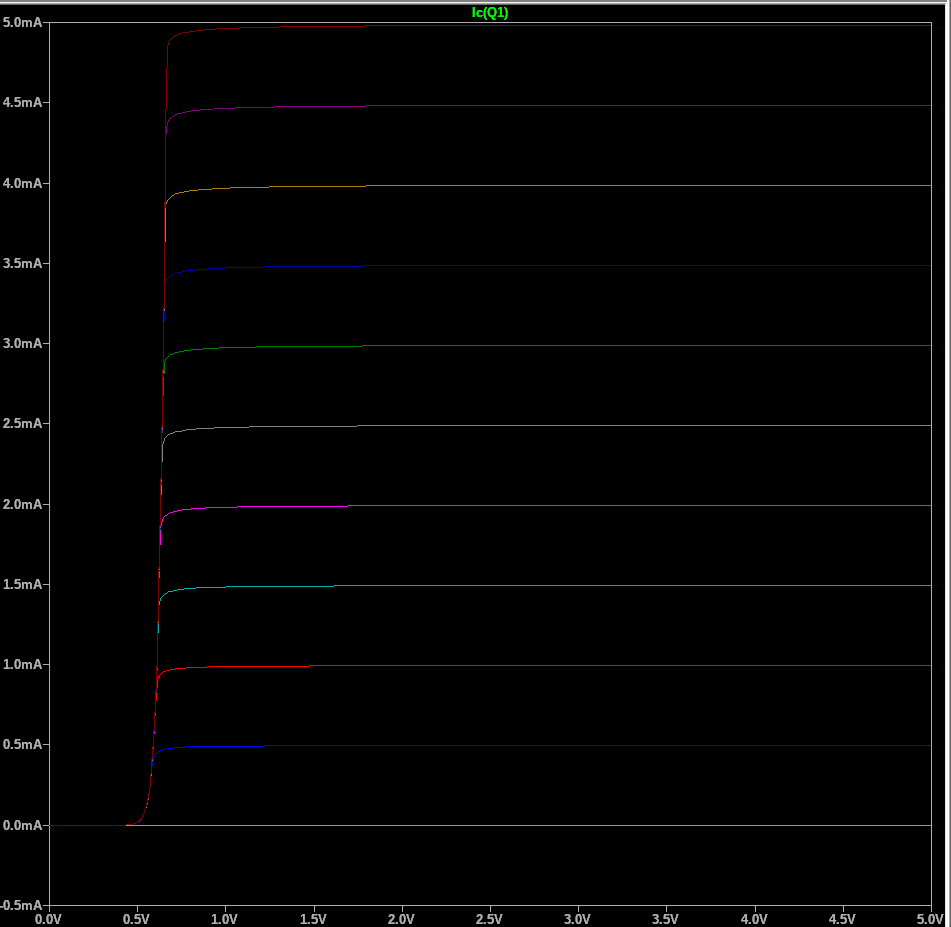
\includegraphics[width=1\linewidth]{figs/bjt-plot.png}
    \end{figure}
    \subsection{Diode}
    \begin{figure}[h!]
        \centering
        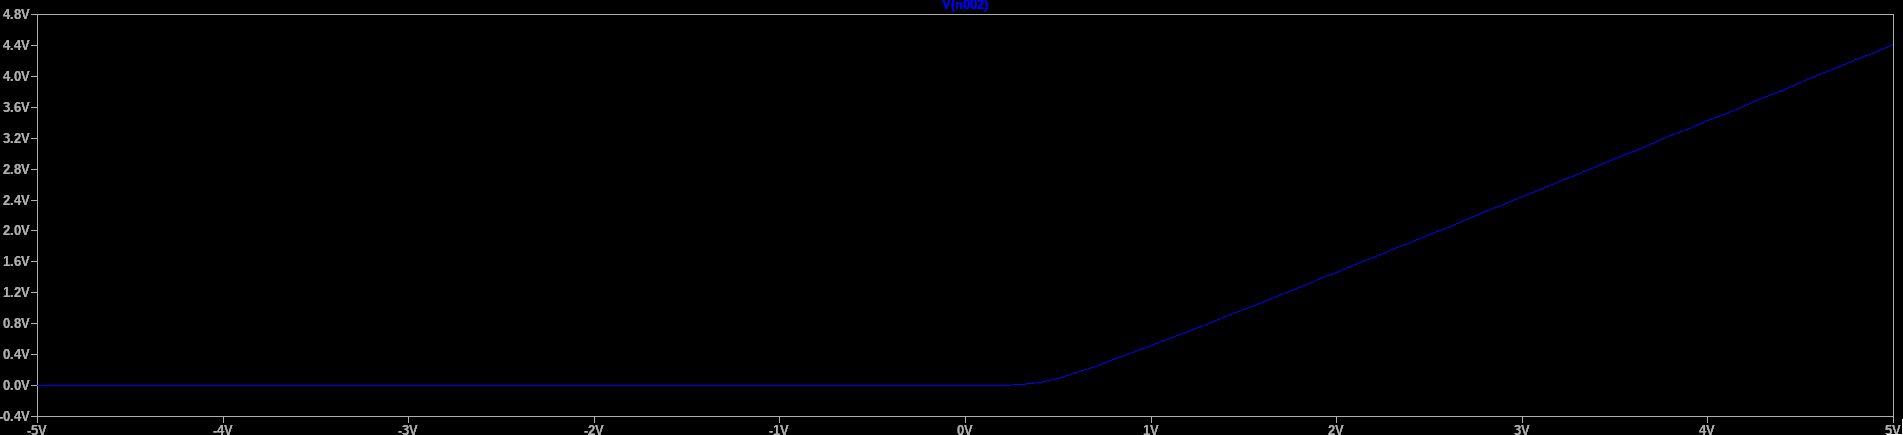
\includegraphics[width=1\linewidth]{figs/diode-plot.png}
    \end{figure}
\section{Conclusion}
VI characteristics of MOSFET, BJT, diode have been plotted using LTspice software.
\end{document}
